\documentclass[a4paper,12pt]{report}

\usepackage[utf8]{inputenc}
\usepackage[T1]{fontenc}
\usepackage[french]{babel}
\usepackage[top=20mm, bottom=25mm, left=15mm, right=15mm]{geometry}
\usepackage{hyperref}
\usepackage{mathpazo}

\usepackage{graphicx}

\usepackage{fancyhdr}

\setlength{\parindent}{3em}
\setlength{\parskip}{1em}

\setcounter{secnumdepth}{3}
\renewcommand{\thesection}{\arabic{section}}
\renewcommand{\thesubsection}{\arabic{section}.\arabic{subsection}}
%\titleformat{\subsubsection}[runin]{\normalfont\bfseries}{\thesubsubsection}{0em}{}

\pagestyle{fancy}
\fancyhead[L]{Projet GE2}
\fancyhead[C]{\textit{Aéroglisseur radiocommandé}}
\fancyhead[R]{Pré-étude - Mars 2020}
\fancyfoot[L]{INSA Strasbourg}
\fancyfoot[R]{Tristan DRUSSEL - Florian POUTHIER}
\headheight=14.5pt

\title{Rapport de Pré-étude Projet GE II\\Aéroglisseur radiocommandé}
\author{Tristan DRUSSEL - Florian POUTHIER \\ \\ Génie Électrique 4ème année\\ INSA Strasbourg}
\date{Année scolaire 2019-2020}

\begin{document}
	\begin{titlepage}
		\maketitle
	\end{titlepage}
	\tableofcontents
	\newpage
	
	\section{Introduction}
	
	\vspace{-1em}
	
	Dans le cadre de notre formation Génie Électrique à l'INSA Strasbourg, le \textbf{projet GE II} du semestre 8 a pour objectif la conception d'un système électrique comprenant des éléments de conversion statique et de commande électronique programmable. Ce projet sera notamment l'occasion de mettre en œuvre nos connaissances acquises en électronique de puissance, en électronique numérique, en informatique industrielle et en automatique tout au long de notre cursus. 
	
	Le thème retenu cette année consiste en une compétition baptisée "La nuit de la glisse". L'objectif sera de présenter pour cette compétition un \textbf{aéroglisseur radiocommandé} qui devra répondre à un certain nombre d'exigences pour pouvoir être homologué et ainsi participer à l'épreuve finale. En vue de réaliser un tel système, nous partirons d'un cahier des charges succinct pour mener une analyse fonctionnelle du dispositif, rédiger un cahier des charges complet et finalement concevoir, simuler, tester et fabriquer l'aéroglisseur attendu.
	
	Ce projet sera également pour nous l'occasion de développer nos compétences linguistiques dans la langue anglaise par le biais de rapports oraux ponctuels lors des différentes étapes de développement du système. Les aspects linguistiques ciblés sont notamment la maîtrise du vocabulaire technique relatif au thème du projet ainsi que la maîtrise de formes classiques comme les formes passives. Nous serons également amenés à travailler avec des documents techniques et des ressources bibliographiques en langue anglaise tout au long du projet.
	
	Le projet intégrera finalement les aspects humains de gestion de projet et de communication orale et écrite. Nous ferons vérifier dans un premier temps nos lettres de motivation et CV, pour ensuite définir une stratégie de projet basée autour d'un planning de travail. Les présentations orales de pré-étude, de définition de solution, d'étude... seront réalisées en salle banalisée et filmées afin d'obtenir un meilleur débriefing sur nos méthodes de communication et sur l'amélioration de celles-ci.
	
	\vspace{-1em}
	
	\section{Cahier des Charges}
	
	\vspace{-1em}
	
	Le Cahier des Charges (CdC) développé ci-dessous va nous servir de base en répertoriant toutes les contraintes à respecter afin de mener à bien notre projet et de proposer un système homologable à la compétition finale. Les contraintes du projet sont multiples, qu'elles soient mécaniques, électroniques ou bien temporelles.
	
	\vspace{-1em}
	
		\subsection{Partie mécanique de l'aéroglisseur}
		
		\vspace{-1em}
		
		La structure de l'aéroglisseur va être le support de tout le développement électronique du projet. Bien que cette partie ne soit pas ciblée dans l'évaluation des compétences mises en oeuvre, il n'en demeure pas moins que l'aéroglisseur doit respecter certaines contraintes évidentes de conception et d'encombrement.
		
		\begin{itemize}
			\item[$\bullet$] Les dimensions de l'aéroglisseur ne devront pas dépasser \textbf{250mm en largeur}, \textbf{350mm en longueur} et \textbf{300mm en hauteur}
			\item[$\bullet$] L'\textbf{hélice de propulsion} devra être \textbf{protégée} et \textbf{ne présenter aucun danger} pour l'environnement extérieur (pilotes, spectateurs, ...)
			\item[$\bullet$] La structure devra permettre de \textbf{porter l'électronique du système} et une \textbf{caméra du type GoPro}
			\item[$\bullet$] Un espace devra également être prévu pour un \textbf{système de coupure générale} qui soit \textbf{facile d'accès} en cas de coupure nécessaire du dispositif
			\item[$\bullet$] La structure devra être réalisée intégralement en \textbf{carton plume}
		\end{itemize}
		
		\vspace{-1em}
		
		\subsection{Contraintes électroniques de l'aéroglisseur}
		
		\vspace{-1em}
		
		Nous allons définir ci-dessous l'ensemble des contraintes électroniques à respecter pour concevoir notre aéroglisseur. Cette partie est le coeur du projet GE II, et nous allons essayer d'établir un cahier des charges fonctionnel le plus exhaustif possible pour proposer un système adéquat avec les attendus du rendu. Ces contraintes peuvent être synthétisées en trois grands axes : les contraintes liées à la \textbf{motorisation}, les contraintes liées à l'\textbf{alimentation} et les contraintes liées à la \textbf{télécommande}.

		\vspace{-1em}		
		
			\subsubsection{Contraintes liées à la motorisation}
			
			\vspace{-1em}
			
			La motorisation des aéroglisseurs permet le déplacement du système en entrainant une hélice qui servira à la fois à la propulsion et à la création du coussin d'air. 
			
			\begin{itemize}
				\item[$\bullet$] La motorisation sera mise en oeuvre par un moteur unique type \textbf{brushless triphasé} de référence \textbf{NM Prodrive 3530 1100kV}
				\item[$\bullet$] Le moteur brushless sera alimenté par un \textbf{onduleur triphasé en pont} commandé par un circuit programmable \textbf{DsPIC30F2010}
				\item[$\bullet$] L'onduleur triphasé sera constitué de \textbf{six transistors MOSFET canal N} \textbf{BSC0902NS} du constructeur \textit{Infineon}
				\item[$\bullet$] Les drivers de demi-pont \textbf{MIC4104YM} de \textit{Microchip} seront utilisés dans le montage
				\item[$\bullet$] Chaque demi-pont sera découplé du bus continu par un \textbf{condensateur de découplage} aluminium polymère 330$\mu F$ 16V de référence \textbf{A750KK337M1CAAE014} du constructeur \textit{Kemet}
				\item[$\bullet$] Le moteur brushless ne disposant pas de capteurs à effet Hall, une \textbf{commande par retour de force électromotrice} devra être implémentée
			\end{itemize}
			
			\vspace{-1em}
			
			\subsubsection{Contraintes liées à l'alimentation}
			
			\vspace{-1em}
			
			L'alimentation du système devra être conçue de manière à pouvoir alimenter tous les éléments électroniques nécessaires au bon fonctionnement du dispositif. Elle doit également répondre à certaines contraintes pour être la plus opérationnelle possible.
			
			\begin{itemize}
				\item[$\bullet$] La source unique d'alimentation sera une \textbf{batterie LiPo 3S 2200 mAh}
				\item[$\bullet$] Les autres niveaux de tensions nécessaires au fonctionnement du dispositif seront générés par des \textbf{convertisseurs DC/DC indépendants}
				\item[$\bullet$] La conversion vers le niveau de tension \textbf{5V} sera réalisée par le régulateur à découpage fixe \textbf{LM22672MR-5.0/NOPB} du constructeur \textit{Texas Instruments}
				\item[$\bullet$] La conversion vers le niveau de tension \textbf{3.3V} sera assurée par le régulateur linéaire \textbf{MCP1826S-3302E/EB} de \textit{Microchip}
				\item[$\bullet$] L'aéroglisseur devra comporter un \textbf{interrupteur général marche arrêt} qui coupera l'alimentation de l'électronique et du moteur
				\item[$\bullet$] Un \textbf{système de coupure générale} permettant de couper l'alimentation globale devra être câblé.
			\end{itemize}
			
			\vspace{-1em}
			
			\subsubsection{Contraintes liées à la télécommande}
			
			\vspace{-1em}
			
			\begin{itemize}
				\item[$\bullet$] L'aéroglisseur sera télécommandé via un \textbf{smartphone} (Android ou iOS) en utilisant une \textbf{liaison Bluetooth}
				\item[$\bullet$] L'application sur la télécommande est libre et peut inclure des joysticks, jauges, boutons ou une gestion de l'inclinaison pour le pilotage de l'aéroglisseur
				\item[$\bullet$] Le module Bluetooth retenu est de type \textbf{HC-05} intégré sur une platine \textbf{zs-040} et assurera la communication entre la télécommande, le servomoteur de direction et l'onduleur du moteur de propulsion
				\item[$\bullet$] Les protocoles de communication entre le récepteur et l'onduleur devront respecter les \textbf{normes des télécommandes de modélisme}
				\item[$\bullet$] Les commandes devront être \textbf{proportionnelles} (au minimum \textbf{5 niveaux} pour la direction et la propulsion)
				\item[$\bullet$] Un \textbf{système de sécurité} sera mis en oeuvre pour arrêter le moteur si l'aéroglisseur ne reçoit \textbf{pas d'information} de la télécommande \textbf{pendant plus de 200ms}
			\end{itemize}
			
			\vspace{-1em}
		
		\subsection{Principales échéances et livrables attendus}
		
		\vspace{-1em}
		
		Un certain rythme de travail est attendu en vue de mener à bien le projet. Des livrables seront à rendre aux différentes étapes du projet afin de se tenir au rythme imposé.
		
			\vspace{-1em}
		
			\subsubsection{Rapports intermédiaires et final}
			
			\begin{itemize}
				\item[$\bullet$] Le rapport de pré-étude comportera une analyse fonctionnelle du dispositif, une identification
complète des paramètres utiles de la source d’alimentation et de la charge, un cahier des charges détaillé, une explication complète du fonctionnement des sous fonctions constituant le montage
				\item[$\bullet$] Le rapport d’étude définira la solution retenue. Le dimensionnement et la justification des choix de la totalité des composants y figurera ainsi que le schéma définitif (aux normes) et les PCB des
cartes électroniques à réaliser
				\item[$\bullet$] Le rapport final reprendra les 2 premiers rapports ainsi que les explications sur la réalisation, les mesures et les tests faits pour valider le fonctionnement du montage
			\end{itemize}
			
			\vspace{-1em}
		
			\subsubsection{Récapitulatif des points recevables}
			
			\vspace{-1em}
			
			La note finale est la moyenne d'une \textbf{note technique} et d'une \textbf{note de compte-rendu}.
			
			\vspace{-1.5em}
			
			\paragraph{Note technique}
			
			Elle est établie à partir du résultat de l'homologation, de la compétition, et de l'évaluation du produit fini :
			
			\begin{itemize}
				\item[$\bullet$] La note technique sera \textbf{inférieure à la moyenne} si l'aéroglisseur ne passe pas les \textbf{épreuves d'homologation} (quelque soit la quantité et la qualité du travail fourni).
				\item[$\bullet$] Une note technique minimale de 12 sera attribuée à tous les participants aux courses. 
				\item[$\bullet$] Les 8 points restants sont divisés en deux parties :
				\begin{itemize}
					\item[$\circ$] Une première partie sur 4 points est liée au nombre de points acquis pendant la compétition
					\item[$\circ$] Une seconde partie sur 4 points est attribuée suivant des critères de réalisation, de programmation, d’esthétique, de fair-play, de pilotage, d’amortissement financier, de gestion du planning, d’originalité...
				\end{itemize}
			\end{itemize}
			
			\vspace{-1.5em}
			
			\paragraph{Note de compte-rendu}
			
			Elle est établie à partir de la note des trois compte-rendus à rendre :
			
			\begin{itemize}
				\item[$\bullet$] Le rapport de \textbf{pré-étude} est noté sur \textbf{3 points}
				\item[$\bullet$] Le rapport d'\textbf{étude} et de fabrication est noté sur \textbf{5 points}
				\item[$\bullet$] Le \textbf{compte-rendu final} est noté sur \textbf{12 points}
			\end{itemize}
			
	\vspace{-1.5em}		
			
	\section{Analyse fonctionnelle du système}
	
	\vspace{-1em}
	
	Suite à l'étude du cahier des charges précédemment exposé, nous devons maintenant mener une analyse fonctionnelle de notre système. Cette analyse doit recenser l'ensemble des dispositifs nécessaires au fonctionnement de notre système et doit montrer comment ces dispositifs sont liés entre eux. Un moyen visuel et concret d'aborder cette analyse est de réaliser un diagramme fonctionnel de notre système. Nous proposons le diagramme fonctionnel électronique de notre aéroglisseur en \textsc{Figure \ref{full_functional}}.
	
	\begin{figure}[h]
		\begin{center}
			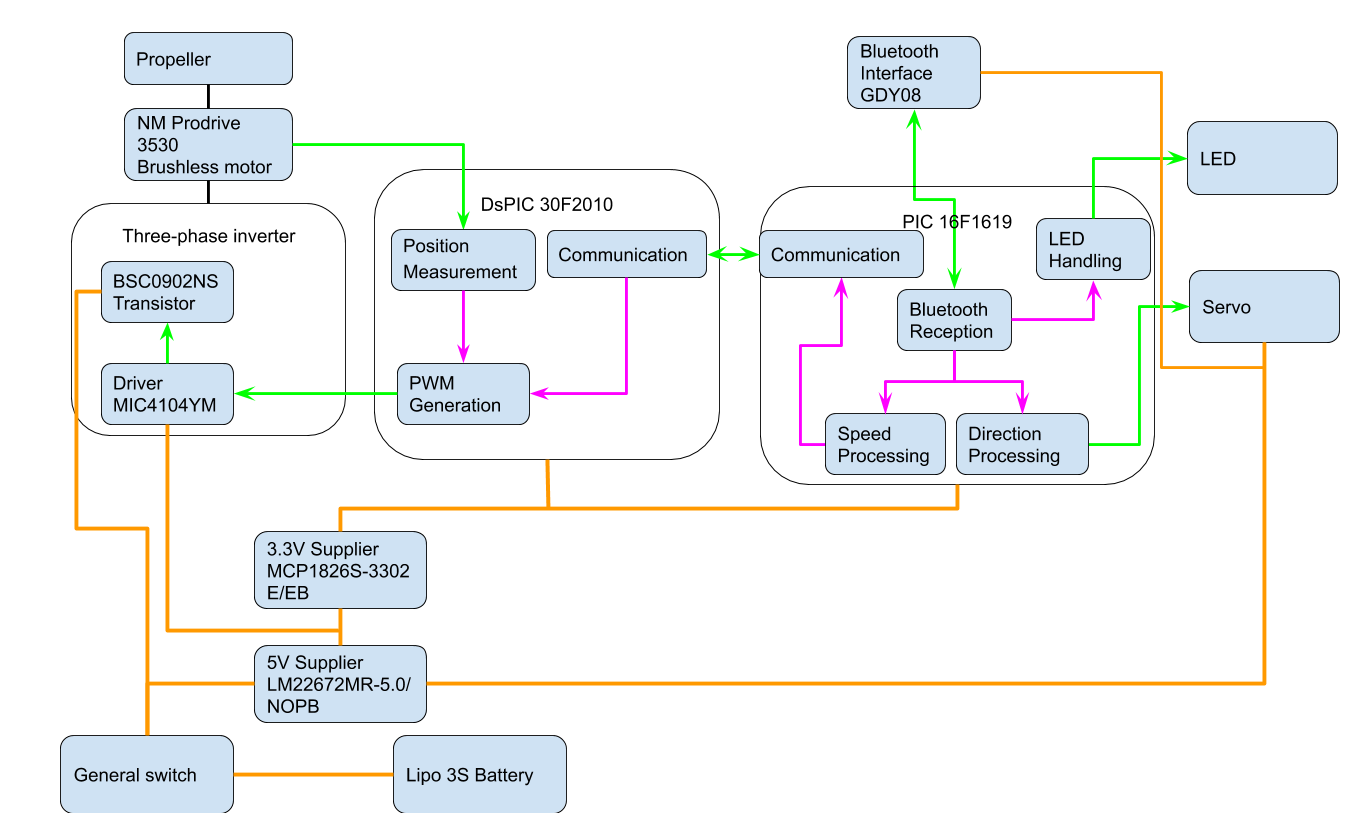
\includegraphics[scale=0.33]{../Illus/full_functional.png}
		\end{center}
		\caption{Diagramme fonctionnel électronique de l'aéroglisseur}
		\label{full_functional}
	\end{figure}
	
	Une fois ce diagramme réalisé, nous avons identifié trois fonctions principales du système que nous pourrons développer sur trois PCB distincts :
	
	\vspace{-0.5em}
	
	\begin{itemize}
		\item[$\bullet$] le \textbf{contrôle de moteur brushless} sera mis en oeuvre sur une première carte. Cette carte comportera le DsPIC30F2010 générant les signaux de PWM, ainsi que les transistors et drivers de demi-pont de l'onduleur triphasé.
		\item[$\bullet$] les différents \textbf{niveaux de tension} nécessaires au fonctionnement du système seront générés sur une seconde carte. Elle comportera les deux régulateurs de tension, qui sont le régulateur à découpage fixe 5V et le régulateur linéaire 3V3.
		\item[$\bullet$] la \textbf{communication Bluetooth} et le \textbf{traitement de la position et de la vitesse de déplacement} de l'aéroglisseur sera développé sur une troisième carte. Elle accueillera entre autre le PIC16F1619 et le module \textit{Bluetooth Low Energy} permettant la communication avec le smartphone utilisé comme télécommande.
		
	\end{itemize}
	
	\section{Développement des sous-fonctions du système}
	
		\vspace{-1em}
	
		L'étape suivante du projet consiste en une étude bibliographique permettant d'en savoir plus sur les différentes sous-fonctions de l'aéroglisseur, et en particulier développer sommairement les aspects technologiques de chacun des dispositifs entrant dans le diagramme fonctionnel.
		
		\vspace{-1em}
		
		\subsection{Contrôle du moteur Brushless DC de propulsion}
		
		\vspace{-1em}
		
			La propulsion de l'aéroglisseur est assurée par une hélice entrainée par un moteur Brushless DC. Ce type de moteur est structuré à partir d’un aimant permanent au rotor et de pôles
bobinés au stator. L’énergie électrique est convertie en énergie mécanique par le biais des forces
d’attraction magnétique entre l’aimant permanent du rotor et le champ tournant induit par les
pôles bobinés du stator. La \textsc{Figure \ref{struct_bldcm}} présente une illustration simplifiée de la construction d’un
BLDCM.
				\begin{figure}[h]
				 	\begin{center}
				 		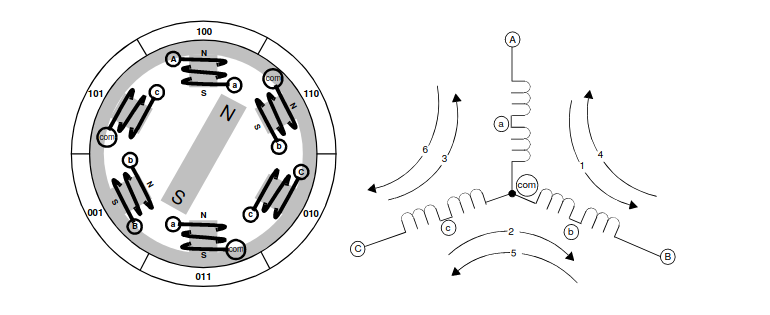
\includegraphics[scale=0.7]{../Illus/struct_bldcm.png}
				 	\end{center}
				 	\caption{Diagramme simplifié de la structure d'un BLDCM (\textit{Source :} \cite{AN857})}
				 	\label{struct_bldcm}
				 \end{figure}
				 
			\vspace{-1em}
				 
			Nous développerons dans le rapport d'étude la caractérisation du moteur \textbf{NM Prodrive 3350 110kV} permettant d'en obtenir un modèle représentatif et pouvoir le contrôler de manière adéquate.
			
			\vspace{-1em}
				 
			\subsubsection{Onduleur triphasé}
			
			\vspace{-1em}
				 
			Afin de piloter ce moteur, nous utiliserons une structure d'onduleur triphasé comme représentée en \textsc{Figure \ref{three_phase_bridge}}. Les MOSFETs retenus pour concevoir cet onduleur sont les \textbf{BCS0902NS}. Ils sont accompagnés dans le montage par des drivers de demi-pont \textbf{MIC4104YM} recevant en entrée les signaux de PWM générés par le \textbf{DsPIC30F2010}.
			
				\begin{figure}[h]
				 	\begin{center}
				 		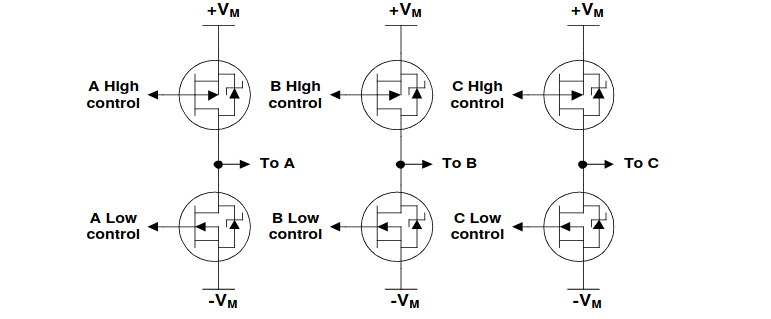
\includegraphics[scale=0.7]{../Illus/three_phase_bridge.png}
				 	\end{center}
				 	\caption{Structure générale d'un onduleur triphasé (\textit{Source :} \cite{AN857})}
				 	\label{three_phase_bridge}
				 \end{figure}	
				 
				 \vspace{-1em}		
			
			\subsubsection{Contrôle basé sur le retour de force électromotrice}
			
			\vspace{-1em}
			
			Il est important de remarquer que le moteur utilisé dans la conception de notre aéroglisseur n'est  équipé ni de capteurs à effet hall ni de codeur incrémental. Il va donc falloir trouver une méthode n'utilisant pas de capteur pour contrôler le moteur.
			
			Afin d'obtenir une information sur la position du rotor du moteur brushless et par conséquent pouvoir le piloter, nous allons devoir utiliser une méthode particulière de contrôle basée sur le \textbf{retour de force électromotrice}. Un schéma générique du montage à réalisé pour mettre en oeuvre cette méthode est exposé en \textsc{Figure \ref{back_emf_scheme}}.	
			
			\begin{figure}[h]
				 	\begin{center}
				 		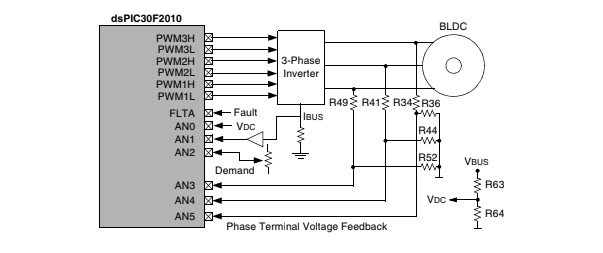
\includegraphics[scale=0.8]{../Illus/back_emf_scheme.png}
				 	\end{center}
				 	\caption{Mise en oeuvre de la méthode de retour de FEM (\textit{Source :} \cite{AN992})}
				 	\label{back_emf_scheme}
				 \end{figure}	
				 
		\vspace{-1em}
				 	
		\subsection{Interface d'alimentation}
		
		\vspace{-1em}
		
		Afin de fonctionner dans son intégralité, le système a besoin de différents niveaux de tension, parmi lesquels un niveau de 5V pour le servomoteur et l'alimentation du driver de demi-pont, et du 3.3V pour l'alimentation des microcontrôleurs et l'utilisation du \textit{Bluetooth Low Energy}. Il est donc prévu de concevoir à cet effet un PCB permettant d'obtenir tous les niveaux de tension nécessaires sur une seule carte et ainsi les distribuer à tous les éléments fonctionnels du système.
		
		\vspace{-1em}
		
			\subsubsection{Caractérisation de la source d'alimentation}
			
			\vspace{-1em}
			
			La source d'alimentation de notre projet est une \textbf{batterie LiPo 3S}. Ce type de batterie est structuré par 3 cellules LiPo de 3.7V en série, soit une \textbf{tension nominale de 11.1V} (3 x 3.7V) pour la batterie LiPo 3S à vide. Un élément LiPo est en fait une batterie Li-ion où l'électrolyte est un polymère gélifié.
			
			Il est à garder en mémoire que la décharge d'un élément LiPo en-dessous de 2.5V entraîne sa destruction. De manière générale, il est recommandé de ne pas décharger les éléments en-dessous de 3.3V si l'on souhaite une durée de vie optimale pour ce type de batterie. 
			
		A l'inverse, chaque élément LiPo \textbf{ne doit jamais être chargé au-dessus de 4.2V}, au risque de provoquer un \textbf{possible incendie}. Dans le cas d'une batterie constituée d'éléments LiPo multiples, il est \textbf{impératif d'utiliser un \textit{égaliseur}} dans le circuit de charge \cite{LiPo}.
		
		\vspace{-1em}
			
			\subsubsection{Conversion tension batterie vers 5V}
			\vspace{-1em}
				
			La conversion depuis le 11.1V de la batterie vers la tension régulée 5V va être réalisée par le composant \textbf{LM22672MR-5.0/NOPB} du constructeur \textit{Texas Instruments}.
			
			\vspace{-1em}
			
			\subsubsection{Conversion 5V vers 3.3V}
			
			\vspace{-1em}
			
			Le composant \textbf{MCP1826S-3302E/EB} de \textit{Microchip} a été retenu pour établir la conversion 5V vers 3.3V. Ce régulateur linéaire fournissant une sortie faible tension et un courant de 1000mA typique a été choisi dans sa version sortie standard fixe 3.3V. Le composant est stable en utilisant en sortie un condensateur céramique de valeur 1uF, ce qui facilite largement son dimensionnement. Seulement une capacité d'entrée sera à déterminer pour mettre en œuvre le régulateur.
			
		\vspace{-1em}
	
		\subsection{Contrôle de la direction}
		
		\vspace{-1em}
		
			L'aéroglisseur doit pouvoir tourner dans toutes les directions pour pouvoir traverser le parcours. La direction s'effectue en orientant la dérive de l'aéroglisseur, celle-ci orientera le flux d'air et ainsi induira un mouvement de rotation à l'ensemble du système. L'actionneur que nous avons pour réaliser le déplacement de la dérive est un servomoteur.
			
		\vspace{-1em}
		
			\subsubsection{Servomoteur}
			
			\vspace{-1em}
			
			Un servomoteur est un moteur asservi en position ou en vitesse. Grâce à un signal de commande caractérisé plus loin, le moteur rejoint une position angulaire ou une vitesse donnée. L'emploi de ce type d'actionneur est simple, une alimentation fixe en 0-5V et un signal de commande permet la réalisation simple de système contrôlé angulairement. Le mot "servo" ne vient pas de cerveau qui signifierait intelligent mais du latin \textit{servus} qui signifie esclave. Il s'agit donc d'un moteur esclave, plus précisément un moteur asservi.
			
			Le signal de commande employé pour contrôler les servomoteurs est un signal de type PWM (Power Width Modulation, Modulation à Largeur d'Impulsion). La largeur de l'impulsion correspond à une position donnée. Le signal est un signal électrique de période 20ms, toutes les 20ms, le moteur doit recevoir un signal de commande pour s'aligner correctement. La largeur de l'impulsion varie généralement entre 0.5 et 3ms. La largeur d'impulsion fait varier proportionnellement l'angle de sortie ou la vitesse. Par exemple, si une impulsion de 0.75ms correspond à un angle de $0^{\circ}$ et une impulsion de 2.25 à un angle de $180^{\circ}$. Pour obtenir un angle de $66^{\circ}$, il faut une impulsion de 1.3ms.   
			
			\vspace{-1em}
			
			\subsubsection{Génération du signal}
			
			\vspace{-1em}
			
			Afin de générer le signal de commande pour le servomoteur, nous allons utiliser le microcontrôleur \textbf{PIC16F1619}. Ce composant programmable nous permettra de générer le signal comportant une impulsion de largeur variable toutes les 20ms. Pour cela, on utilisera un signal PWM de fréquence adaptée, en jouant sur le rapport cyclique, nous jouons sur la largeur de l'impulsion. Cette largeur d'impulsion sera contrôlée par les informations transmises sur la liaison \textit{bluetooth}. En effet, en fonction des commandes envoyées par l'utilisateur, le signal PWM sera ajusté afin d'obtenir la direction de déplacement désirée.
			
		\vspace{-1em}
			
		\subsection{Interface de radiocommande}
			Afin de contrôler la vitesse, la direction et potentiellement d'autres aspects de l'aéroglisseur, nous devons établir une communication entre l'utilisateur et le système. La technologie utilisée dans ce projet est la technologie Bluetooth. Cette technologie a commencé à se déployer en 1998, mais elle a explosé dans les années 2010 avec l'apparition massive des appareils nécessitant une communication à faible distance. Depuis de plus en plus d'appareils utilisent cette technologie qui ne cesse de s'améliorer avec l'apparition par exemple du Low Energy.
			
			\vspace{-1em}
			
			\subsubsection{Module Bluetooth}
			
			\vspace{-1em}
			
			Le module Bluetooth que nous utilisons est le module JDY-08. Ce module permet d'établir une connexion bluetooth avec un autre appareil. Il communique ensuite en USART avec le microcontrôleur PIC16F1619.
			
			\vspace{-1em}
			
			\subsubsection{Application smartphone}
			\vspace{-1em}			
			L'application permettra de réaliser une interface homme-machine entre l'utilisateur et notre aéroglisseur. L'application doit permettre la mise en place d'un protocole précis qui pourra être facilement interprétable par le PIC16F1619. Dans un second temps, l'application doit être ergonomique pour réaliser les différentes fonctions:avancer, tourner et allumer différents effets.
	
	\section{Conclusion}
	
	\vspace{-1em}
	
	Ce rapport de pré-étude a pour objectif de présenter le thème du projet GE II ainsi que les objectifs à atteindre en vue de proposer un système fonctionnel et homologable pour la compétition finale en fin de semestre. Nous y exposons un cahier des charges détaillé, une analyse fonctionnelle du système à réaliser ainsi qu'un développement des sous-fonctions du dispositif à concevoir.
	
	La conception d'un aéroglisseur radiocommandé est un projet d'envergure faisant appel à des notions d'électronique de puissance comme d'électronique numérique. Chaque membre du binôme ayant un attrait plus important pour l'une des deux matières, nous avons décidé de nous répartir la charge de travail par domaine de connaissances. Un des membres du binôme développera alors la partie liée à la communication Bluetooth, la communication entre les différents microprocesseurs tandis que l'autre membre du binôme se concentrera sur la commande du moteur Brushless DC ainsi que la génération des différents niveaux de tension nécessaires au fonctionnement du dispositif.
	
	Ce rapport de pré-étude va ainsi nous donner une solide base d'investigation pour le développement de solutions technologiques fiables et fonctionnelles dans la conception de notre système. Afin d'avoir un meilleur suivi de notre avancée, vous trouverez notre répertoire \href{https://github.com/tristanplouz/ProjetGE2}{github ici}.
	
	\listoffigures
	
	\bibliographystyle{plain} 
	\bibliography{biblio.bib}
	
\end{document}
